


\documentclass[11pt]{article}

\usepackage[utf8]{inputenc} 
\usepackage[T1]{fontenc} 
\usepackage[francais]{babel} 
\usepackage{graphicx}
\usepackage{grffile}
\usepackage{mathpazo} 
\usepackage{indentfirst}
\usepackage[section]{placeins}
\usepackage{url}
\usepackage{hyperref}
\usepackage{geometry}
\usepackage{algorithm}
\usepackage{algpseudocode}
\usepackage{hyperref}
\usepackage{setspace}
\usepackage[tocindentauto]{tocstyle}
\usetocstyle{KOMAlike} %the previous line resets it



\begin{document}




%----------------------------------------------------------------------------------------
%	TITLE PAGE
%----------------------------------------------------------------------------------------

\begin{titlepage}
	\newcommand{\HRule}{\rule{\linewidth}{0.5mm}} 
	
	\center
	
	%------------------------------------------------
	%	Headings
	%------------------------------------------------
	
	\textsc{\LARGE Université Paris Dauphine}\\[1.5cm] 
	
	\textsc{\Large Master 1 MIAGE}\\[0.5cm] 
	

	
	%------------------------------------------------
	%	Title
	%------------------------------------------------
	
	\HRule\\[0.4cm]
	
	{\huge\bfseries Projet de Systèmes \& Algorithmes Répartis}\\[0.4cm]
	
	\HRule\\[2.5cm]
	
	%------------------------------------------------
	%	Author(s)
	%------------------------------------------------
	
	\begin{minipage}{0.4\textwidth}
		\begin{flushleft}
			\large
			\textit{Réalisé par :}\\
			Lyes \textsc{MEGHARA}\\ 
			Vitalina \textsc{MALUSH}\\ 
			Ouerdia \textsc{IDINARENE}\\ 
			Nadia \textsc{MSELLEK}\\ 
		\end{flushleft}
	\end{minipage}
	~
	\begin{minipage}{0.4\textwidth}
		\begin{flushright}
			\large
			\textit{Encadré par :}\\
			Mme Joyce \textsc{EL HADDAD}% Supervisor's name

		\end{flushright}
	\end{minipage}
	

	
	
	\vfill\vfill 
	
	{\large10 Janvier 2018} 
	



	\leavevmode \newline 	\leavevmode \newline 	\leavevmode \newline 	\leavevmode \newline 	\leavevmode \newline 
	
\includegraphics[width=0.6\textwidth]{dauphine.png}\\[1cm] 
	 

	

	
\end{titlepage}


\addtocontents{toc}{\setcounter{tocdepth}{5}} 

\doublespacing

\begingroup
  \hypersetup{hidelinks}
  \tableofcontents
\endgroup

\singlespacing
\clearpage


\renewcommand{\thesection}{\Roman{section}}
\renewcommand{\thesubsection}{\thesection.\Roman{subsection}}

\section{  Introduction}


En nous aidant des procédés et méthodes apprises en cours de Systèmes et Algorithmes répartis, nous avons mis en place un système distribué permettant de créer une simulation boursière.\newline 

Nous avons mis en place un certain nombre d’entreprises souhaitant mettre en vente des actions (dites actions flottantes) sur la bourse,  ainsi que des clients qui eux aussi souhaitent vendre leurs propres actions.\newline D’autres clients souhaitent eux acquérir des actions d’entreprises et sollicitent la bourse qui leur attribue un courtier pour effectuer toutes ces transactions, modélisées par des ordres.




\section{Outils de développement}

Dans le cadre de ce projet, nous avons utilisé GitHub pour une meilleure collaboration, eclipse sous la JDK 1.8, Doxygène nous a permis de générer une documentation visible depuis le fichier index.html. \newline Aussi, l'outil ObjectAid intégré à Eclipse nous a permis de générer automatiquement le diagramme de classes via nos sources, et pour finir ce rapport a été rédigé en utilisant LaTeX.


\section{Description du projet}

\subsection{Hypothèses}

La première hypothèse que nous avons émise est que la bourse est d'abord lancée, s'en suit derrière le(s) courtiers(s) pour enfin lancer les clients. \newline

Aussi, par souci de cohérence avec le fonctionnement des systèmes boursiers avec des clients dans la vie active, le Client envoie 3 ordres successivement en les transmettant à son courtier, qui lui les transmet à la Bourse pour effectuer le traitement, le client attend de recevoir ses réponses avant de décider de ses futures actions (achat/vente). \newline


\clearpage

\subsection{Choix techniques}

Après une réflexion  entre \textit{RMI} et \textit{Socket TCP}, nous avons finalement décidé d'utiliser les Sockets pour les communications entre nos différentes classes; d'une part, c'est un modèle que nous connaissions déjà, et d'autre part, les sockets permettaient d'envoyer et de récupérer des objets (\textit{serializables}) via les objets \textit{ObjectOutputStream} ainsi que \textit{ObjectInputStream} et respectivement les méthodes : \textit{readObject()} et \textit{writeObject()}. \newline 

Aussi, dans un environnement \textit{multi-thread}, l'utilisation des Vector<> a été préviligiée face aux ArrayList<> du fait de leur propriété \textit{safe-thread}. \newline
\newline  Autre chose, pour connaitre l'état du marché, le client possède une \textit{map<NomEntreprise,Prix>} qui correspond donc à \textit{<String,Integer>} le fait de passer le nom de l'entreprise implique la recherche de celle-ci en tant qu'objet pour accéder à ses informations, ce qui impose un détour, néanmoins ce choix nous a paru plus pertinent, car un client n'est pas censé connaitre toutes les informations d'une entreprise juste parce qu'il est un potentiel actionnaire de celle-ci, et que le but de cette map est juste de récupérer le prix de l'action pour chaque (\textit{nom}) entreprise. \newline

Concernant le client cette fois-ci, comme dis explicitement dans l'énoncé, celui-ci lorsqu'il émet un ordre d'achat (resp, de vente) son portefeuille n'est pas réajusté directement, mais uniquement lorsque son courtier reçoit la confirmation de la bourse, pour rester en cohérence avec la vie réelle, celui si prend compte de l'ordre qu'il vient de passer, et enregistre cette dépense éventuelle pour en prendre acte lors de ses futurs achats, l'introduction de l'attribut \textit{depensesEventuelles} (resp \textit{quantiteEventuelleVendu}) nous a permis d'implémenter cette situation, ces derniers sont aussi utilisés dans les méthodes \\ \textit{achatLegal()} et \textit{VenteLegal()} .

\subsection{Pseudo code}

	\begin{algorithm}
		\caption{Client : Produit un ordre}
		\label{Produire un ordre}
		\begin{algorithmic}[0]
			\Procedure{Produire}{$Ordre$}

			\State $EnvoyerA(Courtier,Ordre)$


			\EndProcedure
		\end{algorithmic}
	\end{algorithm}

	\begin{algorithm}
		\caption{Client : Transmet un ordre au courtier}
		\label{Transmet un ordre}
		\begin{algorithmic}[0]
			\Procedure{EchangeOrdreClientCourtier}{)}

			\For {each Ordre $o$ in $ListOrdres$}
				\State $Produire(o)$
			\EndFor
			\State $Attendre($Délai$)$
			
			\For {each Ordre $o$ in $ListOrdres$}
				\State $RecevoirReponse()$
			\EndFor
			\State $Deconnexion()$

			\EndProcedure
		\end{algorithmic}
	\end{algorithm}	


	\begin{algorithm}
		\caption{Courtier : Transmet un ordre au courtier a la bourse}
		\label{Transmet un ordre a la bourse}
		\begin{algorithmic}[0]
			\Procedure{Transmettre}{$Ordre$}
			\State $Envoyer_ABourse(Ordre)$

			\EndProcedure
		\end{algorithmic}
	\end{algorithm}	


	\begin{algorithm}
		\caption{ThreadBourse : Transmet un ordre}
		\label{Transmet un ordre}
		\begin{algorithmic}[0]
			\Procedure{SurReceptionDe}{$Ordre$}
			\State $AjouterALaListedeBourse(o)$
			\State $AjouterALaListeEntreprise(o)$
			\State $if$ (OrdreAchat) IncDemandesAchats
			\State $else$ IncDemandesVentes
			\EndProcedure
		\end{algorithmic}
	\end{algorithm}	

	\begin{algorithm}
		\caption{Bourse  : Consommer un ordre}
		\label{Consommer un ordre}
		\begin{algorithmic}[0]
			\Procedure{Consommer }{$nomCourtier$}
			\For {each Ordre $o$ in $ListOrdres$}
			\State $if$ (Ordre ProvientDe $nomCourtier$)
			\State $SupprimerDeLaListe($Ordre$)$
			\State $renvoyer( $Ordre$)$
			\State $endif$
			\EndFor
			\EndProcedure
		\end{algorithmic}
	\end{algorithm}	


	\begin{algorithm}
		\caption{Bourse  : Accord}
		\label{Consommer un ordre}
		\begin{algorithmic}[0]
			\Procedure{Accord }{$nomCourtier$}
			\State $Consommer$ ($nomCourtier$)
			\State $RepondreAuxDeuxCourtiers()$
			\EndProcedure
		\end{algorithmic}
	\end{algorithm}	


\section{Graphe de communication}

\phantom \\ 
\phantom \\ 
\phantom \\ 
\phantom \\ 
\phantom \\ 
\phantom \\ 

\begin{figure}[!htb]
  \centering
    \caption{Graphe de communications}
    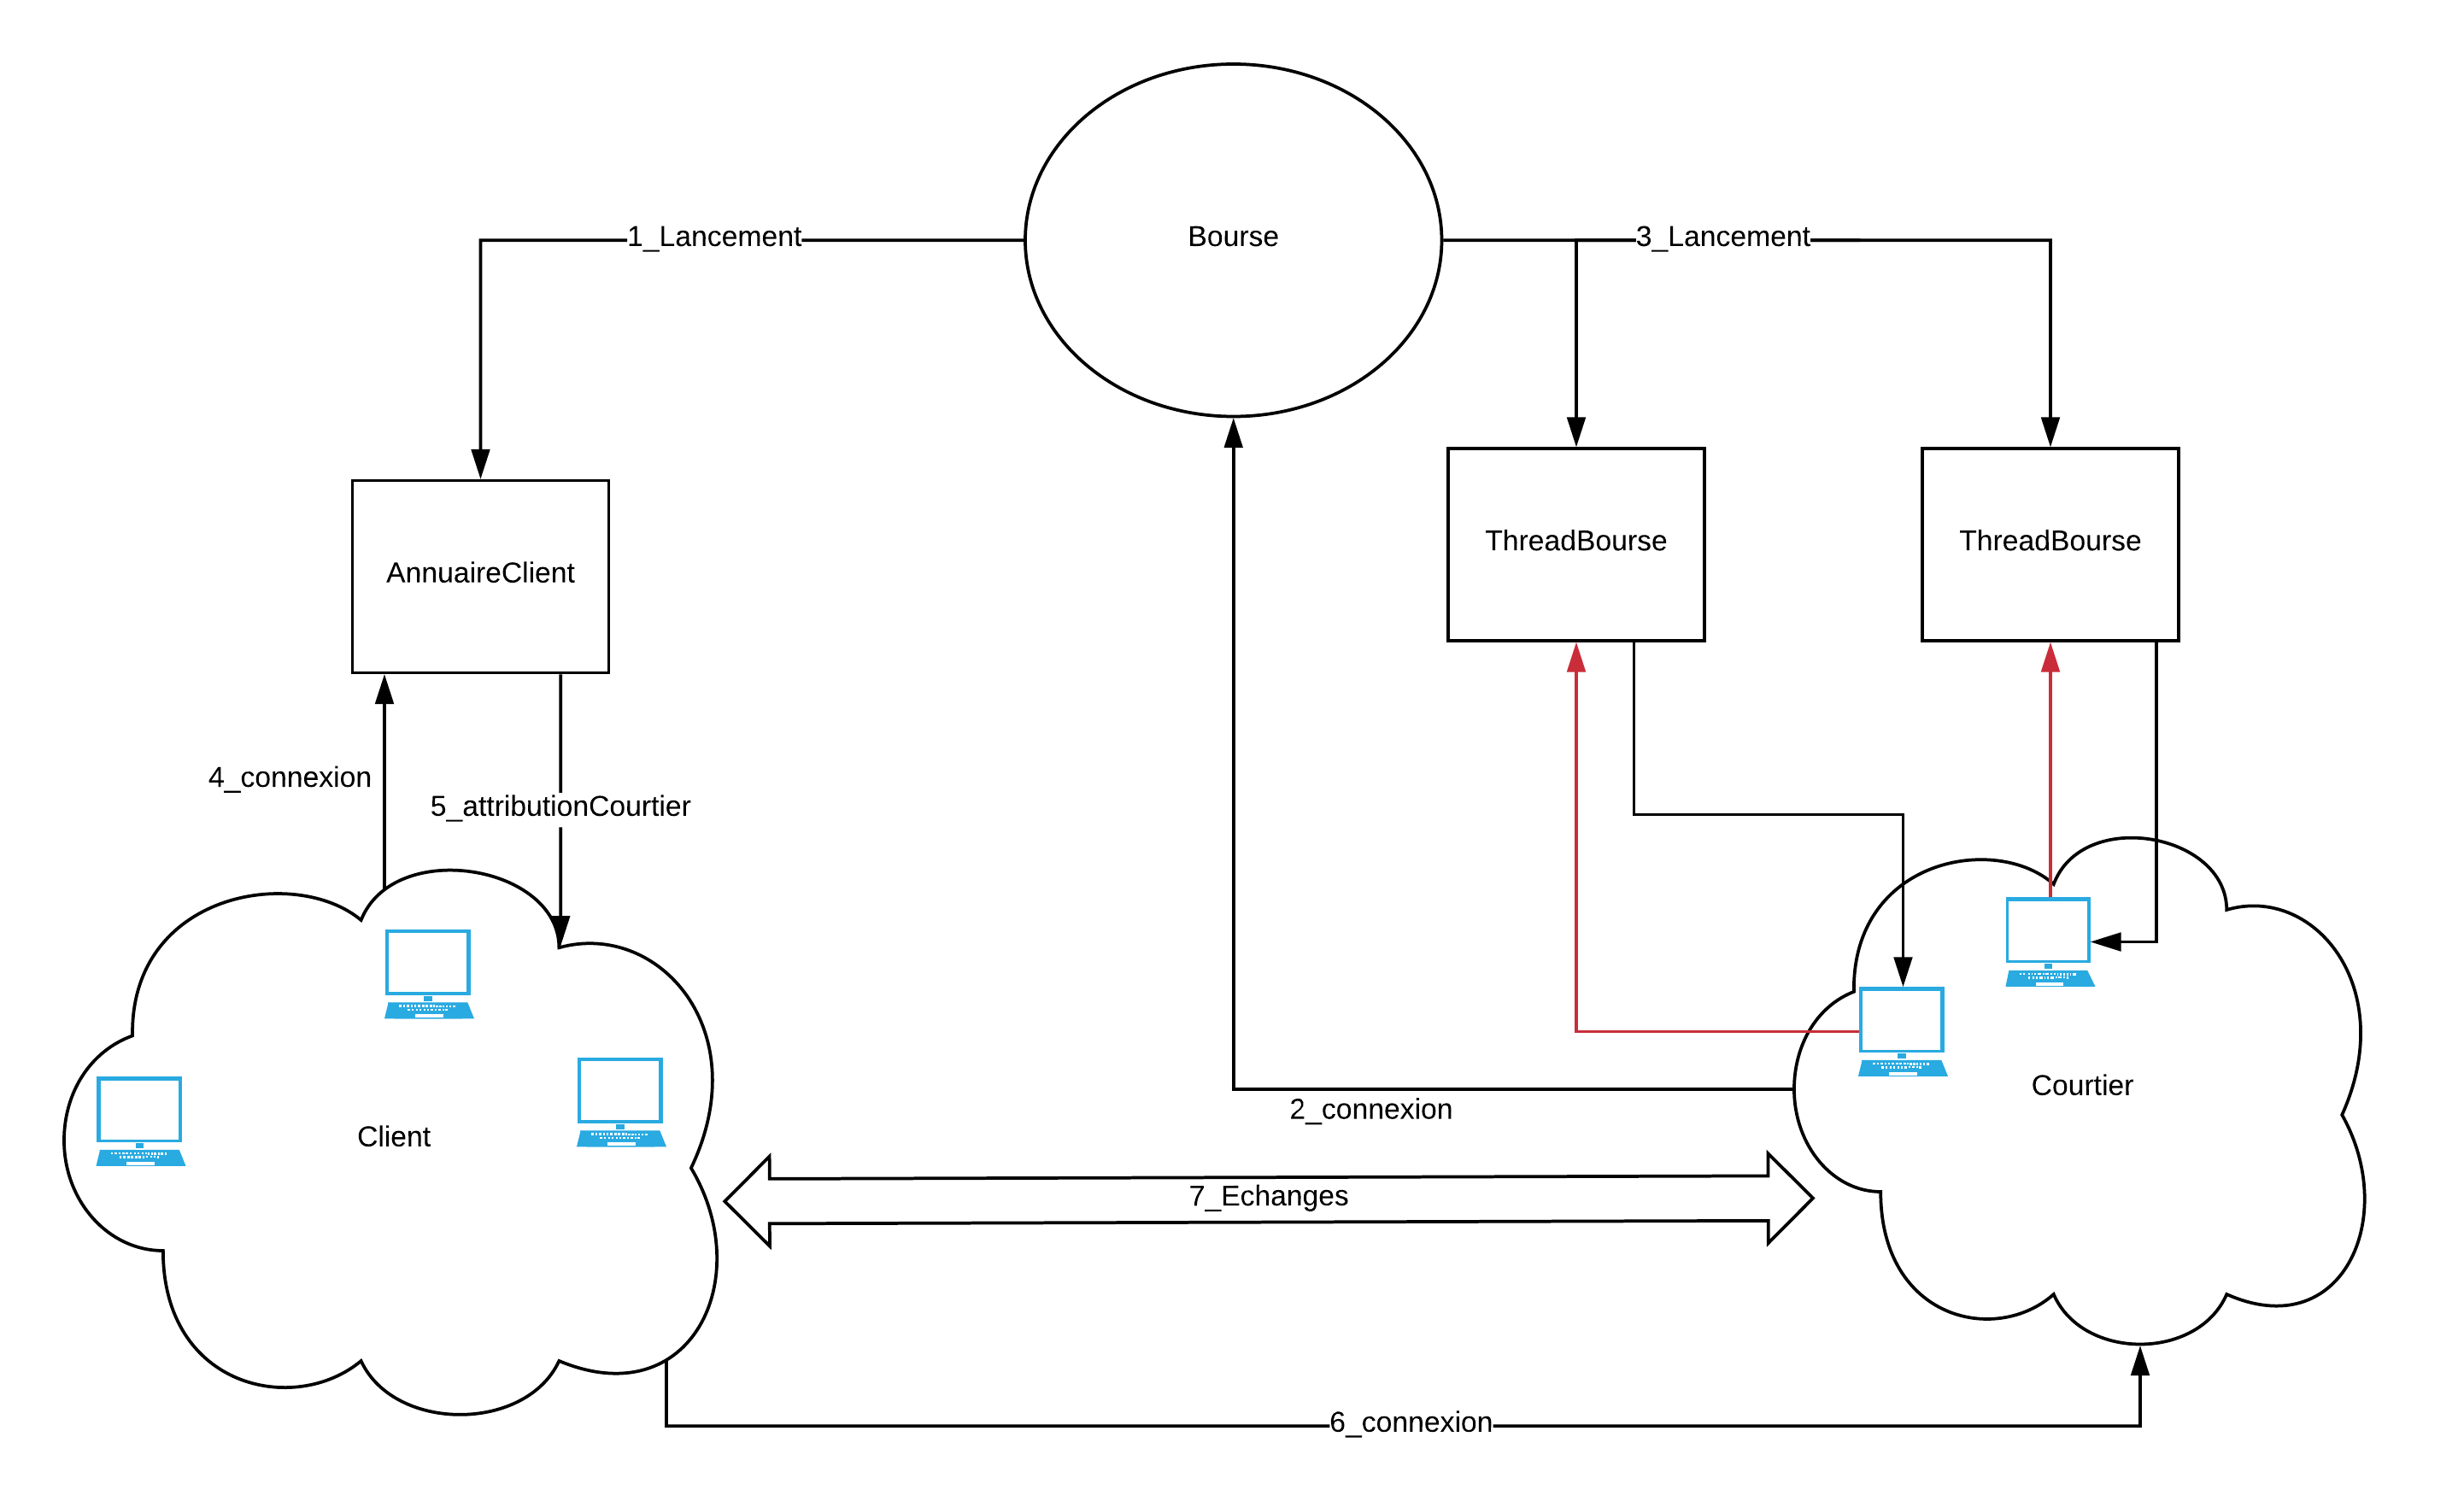
\includegraphics[width=\textwidth]{communication.png}
\newline \newline
\end{figure}

\phantom \\ 
\phantom \\ 
\phantom \\ 
\phantom \\ 
\phantom \\ 

\section{Diagramme de classe}

\begin{figure}[!htb]
  \centering
    \caption{Diagramme de classe tel que généré par ObjectAid}
    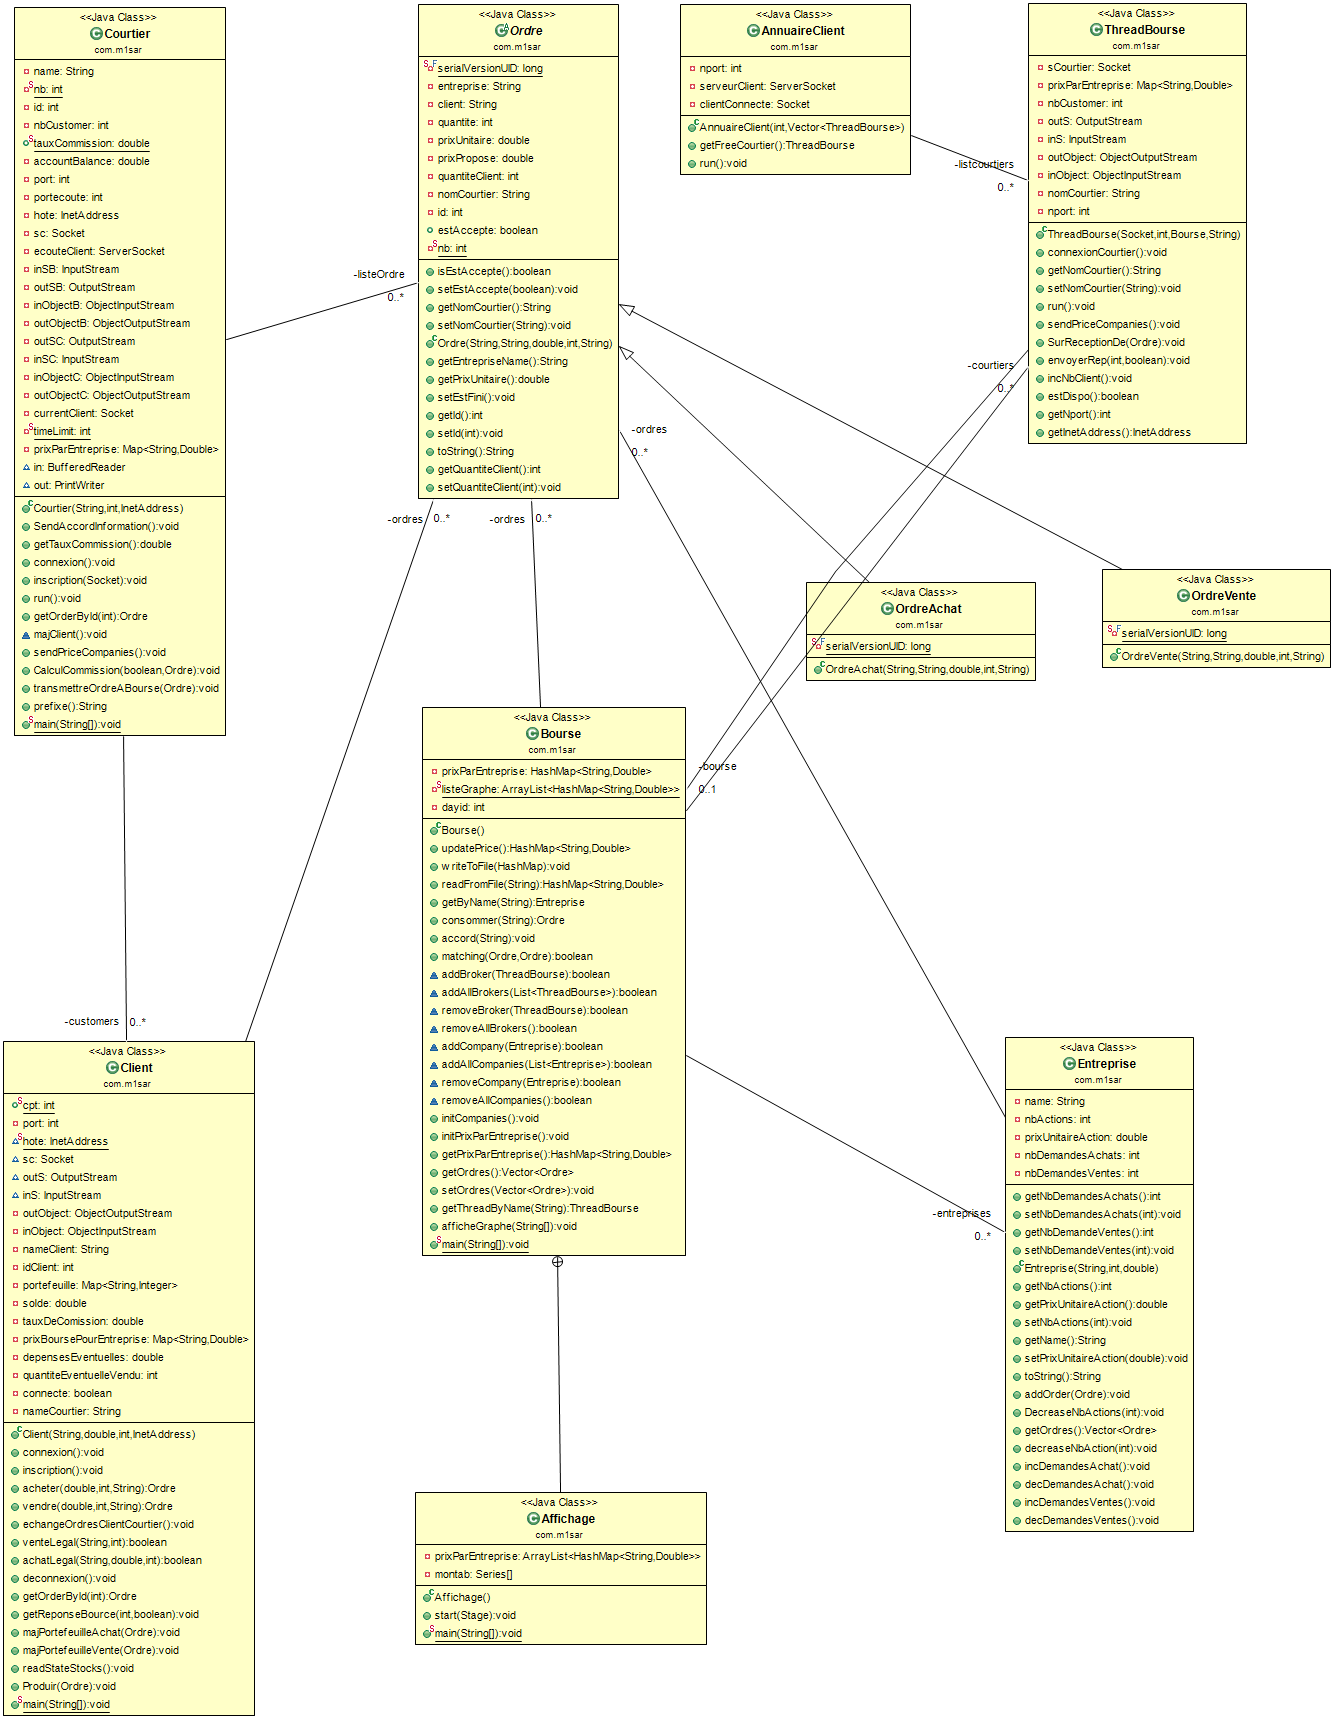
\includegraphics[width=\textwidth]{ClassDiagram.png}
\newline \newline
\end{figure}


\section{Nos initiatives}

Dans le but d'aller plus loin, nous avons intégré un affichage représentant le cours d'évolution des prix par entreprise, et selon les jours, cet affichage est réalisé avec \textit{JavaFX}, et fait partie, en tant que classe interne de la classe Bourse. \newline

\begin{figure}[!htb]
  \centering
    \caption{Courbes représentant l'évolution des prix}
    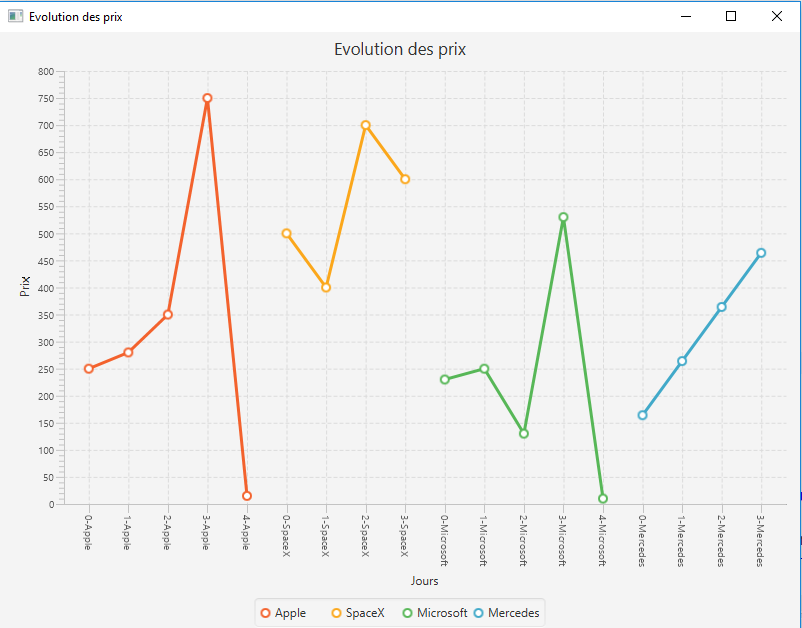
\includegraphics[width=\textwidth]{courbes.png}
\newline \newline
\end{figure}

Aussi, nous voulions tirer parti des avantages des systèmes répartis en mettant en place une politique de panne, le principe auquel nous avions pensé est le suivant : la bourse (serveur principal) détecte (\textit{catch}) une exception, et se met donc à lancer un serveur secondaire, dans ce catch la bourse génère un clone d'elle même (interface \textit{cloneable}), et le relance (\textit{invoke}) via son main. \newline

Cependant, lors de la coupure de cet objet actuel, les connexions avec les autres acteurs (Clients, Courtiers ...) Est aussi interrompu, l'objet cloné et relancé ne les récupère pas, car ces derniers génèrent à leurs tours des exceptions du à la connexion interrompue. \newline

Une \textit{API }trouvée sur \href{https://github.com/jhalterman/failsafe}{GitHub} nous semblait pouvoir pallier efficacement à ce problème, mais nous en sommes restés là par manque de temps.\\
Pour garder un historique des prix et de leurs évolutions, ces derniers sont \textit{serializés} dans des fichiers à la fin de chaque journée, via la méthode \textit{writeToFile()} .


\section{Scénario d'éxecution}



\subsection {Manuel d'utilisation}

Il convient d'abord de compiler les classes, pour ce faire, sur un environnement Linux, lancer simplement compile.sh (chmod + x peut-être nécessaire)\\
Sur un environnement Windows, lancer compile.exe. \\
Une fois la compilation faite, il suffit de lancer les programmes dans l'ordre suivant : \\ \\
Bourse [NPort] \\
Courtier [NPort] [IP] \\
Client [NPort] [IP] \\ \\
IP peut correspondre à localhost dans le cas d'une exécution en local.

\subsection {Phase de connexion}

Un client se connecte d’abord à l’annuaire que publie la bourse où un courtier lui est affecté ensuite ,le client se connecte  à ce courtier. \\ \\
1-Lancer la bourse avec un numéro de port p1=4000. \\
2-Lancer un courtier “James” en spécifiant le numéro de port p1=4000 et @IP de la bourse.\\
3-Lancer un autre courtier “Mario” en spécifiant  le numéro de port p1=4000 et @IP de la bourse.\\
4-Lancer un client “Jack” en spécifiant le numéro de port p2=4001 et @IP de la bourse.\\
5-Lancer un client “Rose” en spécifiant le numéro de port p2=4001 et @IP de la bourse.\\
6-Lancer un client “Eva” en spécifiant le numéro de port p2=4001 et @IP de la bourse.\\
7-Lancer un client “Toto” en spécifiant le numéro de port p2=4001 et @IP de la bourse.\\ 


\subsection {Phase d'échanges}

Hypothèses : Le client peut envoyer autant d’ordres qu’il veut, deux par deux, c’est à dire, il envoie deux ordres, ensuite attends la réponse de la bourse pour envoyer la suite. \\
Le courtier accepte deux clients à la fois, mais traite ces clients séquentiellement. \\

Éva crée 4 ordres :        \\      
un ordre d’achat : a,prix=15,quantité=2,entreprise=Apple \\
Jack crée 5 ordres :  \\
un ordre d’achat : a,prix=15,quantité=3,entreprise=Apple \\
Jack crée un ordre d’achat : a,prix=10,quantité=3,entreprise=Microsoft  \\
Éva crée un ordre d’achat : a,prix=6,quantité=2,entreprise=Ubisoft  \\
Éva crée un ordre d’achat : a,prix=10,quantité=1,entreprise=Microsoft \\
Jack crée un ordre de vente: v,prix=15,quantité=50,entreprise=Apple \\
Jack crée un ordre de vente :v,prix=9,quantité=2,entreprise=Microsoft \\
Éva crée un ordre d’achat :a,prix=9,quantité=2,entreprise=Microsoft   \\
Éva reçoit les réponses : ces ordres d’achat sont validés  \\
Déconnexion d’Eva  \\
Jack crée un ordre de vente :v,prix=10,quantité=2,entreprise=Apple  \\
Déconnexion de Jack  \\
un ordre d’achat : a,prix=15,quantité=3,entreprise=Apple  \\
Rose ne crée aucun ordre (ordre=0)  \\
déconnexion de James et Mario  \\
La bourse incrémente la journée et met à jour les prix des entreprises en prenant en compte le nombre des ordres émis pour chaque entreprise.  \\

\section {Captures d'écran}

\begin{figure}[!htb]
  \centering
    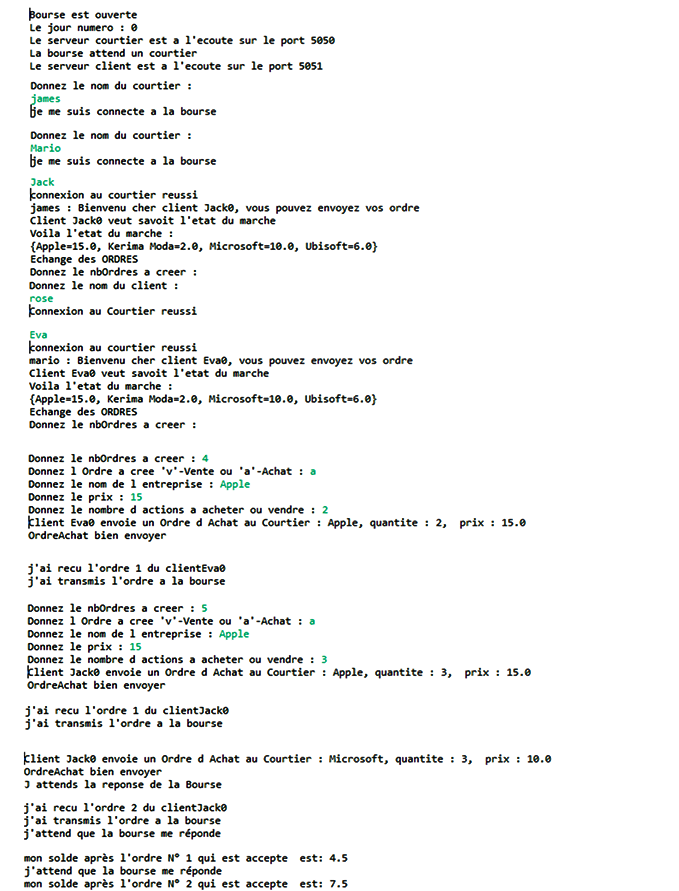
\includegraphics[width=\textwidth]{screen1.png}
\end{figure}

\begin{figure}[!htb]
  \centering
    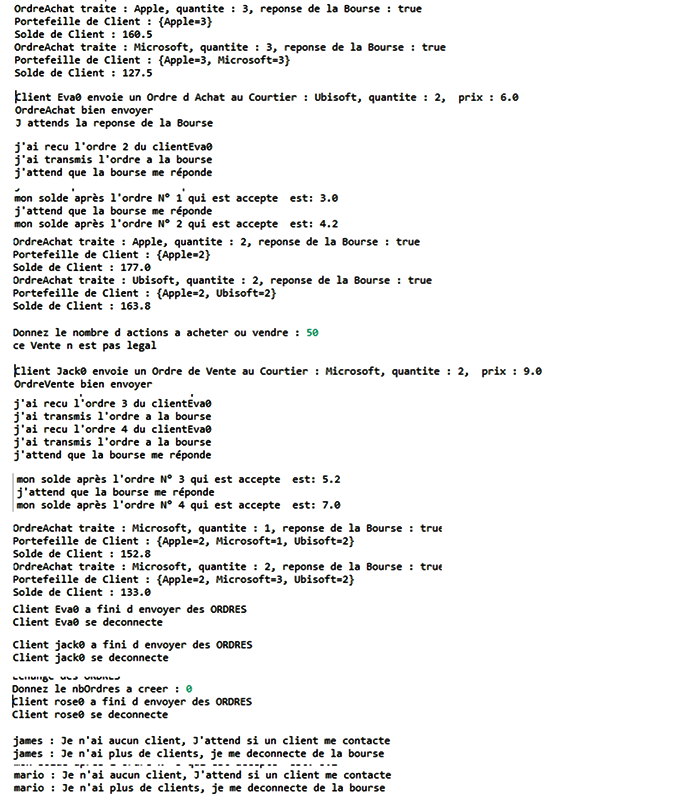
\includegraphics[width=\textwidth]{screen2.png}
\end{figure}
\end{document}
